\section{ХОД РАБОТЫ}

\subsection{Программа определения элемента списка по номеру}

Задание: разработать программу, определяющую элемент списка по его номеру.
Номер задается как аргумент.

Исходный код разработанной программы представлен на
рисунке~\ref{lst:el_by_idx}.

\lstinputlisting[style=source_code,numbers=left,numberstyle=\texttt,xleftmargin=2em,
                 caption=Исходный код программы,
                 language=prolog,label=lst:el_by_idx]{code/el_by_idx.pro}

Пример работы программы представлен на рисунке~\ref{fig:el_by_idx}.

\begin{figure}[h!]
  \centering
  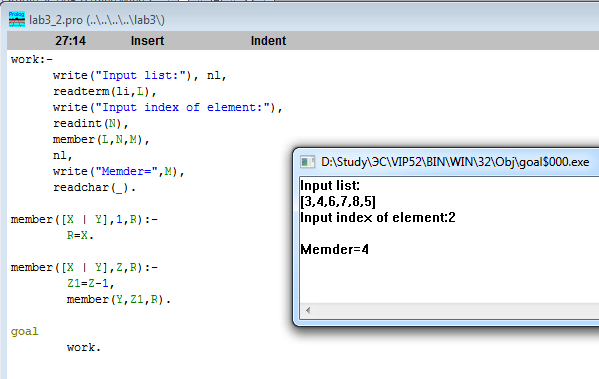
\includegraphics[width=92mm]{img/el_by_idx}
  \caption{Результат работы программы}
  \label{fig:el_by_idx}
\end{figure}


\subsection{Программа определения номера элемента в списке}

Задание: разработать программу, выдающую номер заданного элемента в списке.

Исходный код разработанной программы представлен на
рисунке~\ref{lst:idx_by_el}.

\lstinputlisting[style=source_code,numbers=left,numberstyle=\texttt,xleftmargin=2em,
                 caption=Исходный код программы,
                 language=prolog,label=lst:idx_by_el]{code/idx_by_el.pro}

Пример работы программы представлен на рисунке~\ref{fig:idx_by_el}.

\begin{figure}[h!]
  \centering
  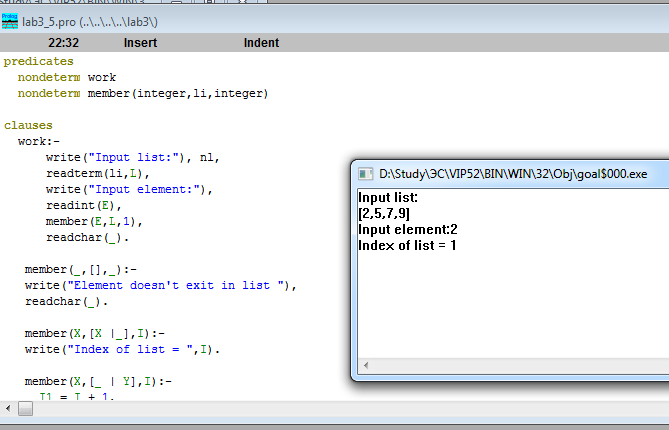
\includegraphics[width=92mm]{img/idx_by_el}
  \caption{Результат работы программы}
  \label{fig:idx_by_el}
\end{figure}


\subsection{Программа определения упорядоченности списка по \\ возрастанию}

Задание: разработать программу, определяющую,
упорядочен ли введенный список по возрастанию.

Исходный код разработанной программы представлен на
рисунке~\ref{lst:is_growing}.

\lstinputlisting[style=source_code,numbers=left,numberstyle=\texttt,xleftmargin=2em,
                 caption=Исходный код программы,
                 language=prolog,label=lst:is_growing]{code/is_growing.pro}

Пример работы программы представлен на рисунке~\ref{fig:is_growing}.

\begin{figure}[h!]
  \centering
  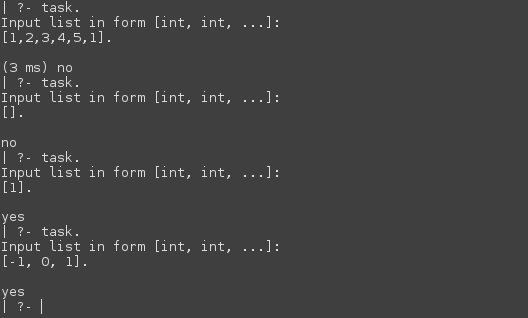
\includegraphics[width=120mm]{img/is_growing}
  \caption{Результат работы программы}
  \label{fig:is_growing}
\end{figure}

Опишем подробно реализацию программы.
Стартовым предикатом в данной программе является предикат \texttt{task}.
Он выводит приглашение ввести список, считывает его и передает в предикат
\texttt{is\_growing} (строки 11-13).

Рассмотрим случай, когда пользователь вводит пустой список. 
В этом случае выполняется предикат \texttt{is\_growing([])}.
Так как такой предикат не определен, то программа возвращает значение \texttt{no}.

В случае, если пользователь вводит список, состоящий из одного элемента, 
например, \texttt{[10]}, то в этом случае выполняется предикат \texttt{is\_growing([\_])},
возвращающий значение \texttt{true} (строка 1). 
Восклицательный знак в теле предиката используется для указания
интерпретатору не пытаться использовать прочие предикаты для унификации.

Наконец, если пользователь вводит список наподобие \texttt{[1,0,-1]},
то выполняется предикат \texttt{is\_growing([1,0,-1])} (строки 2--7). 
Он использует вспомогательный предикат~\texttt{cmp(A, B)}, 
возвращающий \texttt{true} в случае, если A больше B.
Сам предикат \texttt{is\_growing} производит двоекратное отсечение головы
у списка-аргумента, производит их сравнение посредством предиката \texttt{cmp},
затем рекурсивно запускает себя, передавая в качестве аргусмента собственный
аргумент без первого элемента. 
Процесс продолжается до тех пор, пока предикат \texttt{cmp} не вернет \texttt{false},
или мы не дойдем до конца списка.

Приведем последовательность обработки списка \texttt{[1,0,-1]} предикатом \texttt{is\_growing}:

\begin{enumerate}
\item \texttt{is\_growing([1,0,-1]).}
\item \texttt{cmp(1,0).}
\item \texttt{is\_growing([0,-1]).}
\item \texttt{cmp(0,-1).}
\end{enumerate}

Последний предикат возвращает \texttt{false}, 
поэтому предикаты \texttt{is\_growing} и \texttt{task} также возвращает \texttt{false},
таким результатом работы программы является значение \texttt{no}.

\pagebreak

\subsection{Программа определения минимального элемента в списке}

Задание: разработать программу, определяющую
минимальный элемент в списке.

Исходный код разработанной программы представлен на
рисунке~\ref{lst:min_element}.

\lstinputlisting[style=source_code,numbers=left,numberstyle=\texttt,xleftmargin=2em,
                 caption=Исходный код программы,
                 language=prolog,label=lst:min_element]{code/min_element.pro}

Пример работы программы представлен на рисунке~\ref{fig:min_element}.

\begin{figure}[h!]
  \centering
  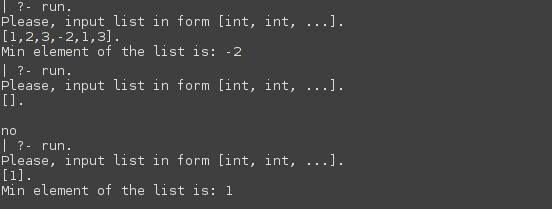
\includegraphics[width=120mm]{img/min_element}
  \caption{Результат работы программы}
  \label{fig:min_element}
\end{figure}

Опишем подробно реализацию программы.
Стартовым предикатом в данной программе является предикат \texttt{run}.
Он выводит приглашение ввести список, считывает его и передает в предикат
\texttt{find\_min}, а затем печатает результат его обработки,
помещенный в переменную \texttt{Min} (строки 13--17).

Рассмотрим случай, когда пользователь вводит пустой список. 
В этом случае выполняется предикат \texttt{find\_min([])}.
Так как такой предикат не определен, то программа возвращает значение \texttt{no}.

В случае, если пользователь вводит список, состоящий из одного элемента, 
например, \texttt{[10]}, то в этом случае выполняется предикат \texttt{find\_min([\_])},
возвращающий значение \texttt{true} (строка 7). 

Для обработки нетривиальных случаев используется предикаты \texttt{cmp(X, Y, Z)}.
Они устанавливают значение переменной Z равным минимальному из \texttt{(X, Y)}.
Оператор отсечения используется в данных предикатах с целью оптимизации.

Если пользователь вводит список наподобие \texttt{[1,0,-1,3]},
то выполняется предикат \texttt{find\_min([1,0,-1,3])} (строки 9--11). 
Он производит рекурсивный вызов, передавая в качестве аргумента
собственный аргумент-список без первого элемента. 
Этот процесс повторяется до тех пор, 
пока в списке аргументе не останется всего один элемент.
Тогда выполняется предикат \texttt{find\_min} (строка 7),
устанавливающий свой второй аргумент равным единственному элементу списка.
Далее производится переход к <<родительским>> функциям, 
но уже с определенным значеним переменной \texttt{Ret}.
В строке 11 производится его сравнение с оторванным ранее элементом списка.
Так как предикат \texttt{cmp} помещает минимальный из первых двух аргументов
в третий, к концу вычисления в переменной \texttt{Min} находится наиментший элемент списка.

Приведем последовательность обработки списка \texttt{[1,0,1]} предикатом \texttt{find\_min}:
\begin{enumerate}
\item \texttt{find\_min([1,0,1], Min).}
\item \texttt{find\_min([0,1], Min).}
\item \texttt{find\_min([1], 1).}
\item \texttt{cmp(0, 1, 0).}
\item \texttt{cmp(1, 0, 0).}
\item \texttt{cmp([1,0,1], 0).}
\end{enumerate}
